\documentclass[12pt]{article}

\usepackage{sbc-template}
\usepackage{graphicx,url}
\usepackage[utf8]{inputenc}
\usepackage[brazil]{babel}
\usepackage{lipsum}
%\usepackage[latin1]{inputenc}  
\usepackage{amsmath}
\usepackage[portuguese,ruled,vlined]{algorithm2e}
%\usepackage[portuguese,ruled,vlined,linesnumbered]{algorithm2e}
\usepackage{blindtext}
\usepackage{xcolor}
\usepackage{caption}
\usepackage{subcaption}
\usepackage{colortbl}
\usepackage{adjustbox}
     
\sloppy

\title{Componentes Conexos em Processador Multicore}
\author{Patreze A. Chita \inst{1}, Nahri. B. Moreano\inst{1}}
\address{Faculdade de Computação -- Universidade Federal do Mato Grosso do Sul (UFMS) \\ Caixa Postal 549 -- 79.070.900 -- Campo Grande -- MS -- Brazil
\email{patrezechita@gmail.com, nahri@facom.ufms.br}
}

\begin{document} 

\maketitle

\begin{abstract}
  This meta-paper describes the style to be used in articles and short papers
  for SBC conferences. For papers in English, you should add just an abstract
  while for the papers in Portuguese, we also ask for an abstract in
  Portuguese (``resumo''). In both cases, abstracts should not have more than
  10 lines and must be in the first page of the paper.
\end{abstract}
     
\begin{resumo} 
  Este meta-artigo descreve o estilo a ser usado na confecção de artigos e
  resumos de artigos para publicação nos anais das conferências organizadas
  pela SBC. É solicitada a escrita de resumo e abstract apenas para os artigos
  escritos em português. Artigos em inglês deverão apresentar apenas abstract.
  Nos dois casos, o autor deve tomar cuidado para que o resumo (e o abstract)
  não ultrapassem 10 linhas cada, sendo que ambos devem estar na primeira
  página do artigo.
\end{resumo}

\section{Introdução}
{\color{gray}\lipsum[1]}

\section{Algoritmo Sequencial e Paralelo para Componentes Conexos}
{\color{gray}\lipsum[1]}

\subsection{Algoritmo Sequencial Baseado em Busca em Profundidade}

{\color{gray}\lipsum[1]}

\begin{algorithm}[H]
    \DontPrintSemicolon
    \caption{Implementação do Algoritmo Sequencial para C. C.}
    \SetKwProg{ComponentesConexos}{sequencialDFS}{}{}
    \ComponentesConexos{$(G=(V,\ A))$}
	{
        $nComponente \gets 0$\;
        $visitado[v] \gets FALSO \mid \forall v \in V$\;
        %$visitado[v] \gets FALSO,\ \{ \forall\ v \mid v \in V\}$\;
        %\ParaCada{$v\acute{e}rtice\ u \in V$}
        %{
        %    $visitado[u] \gets FALSO$\;
        %}
    
        \ParaCada{$v\acute{e}rtice\ v \in V$}
        {
            \Se{$visitado[v] = FALSO$}
            {
                $\textbf{DFS}(v)$\;
                $nComponente \gets nComponente + 1$\;
            }
        }
    }
    
    \SetKwProg{DFS}{DFS}{}{}
    \DFS{$(v\acute{e}rtice\ v)$}
    {
        $componente[v] \gets nComponente$\; 
        $visitado[v] \gets VERDADEIRO$\;
        \ParaCada{$v\acute{e}rtice\ u \in Adj[v]$}
        {
            \Se{$visitado[u] = FALSO$}
            {
                $\textbf{DFS}(u)$\;
            }
        }
    }
\end{algorithm}

\subsection{Algoritmo Paralelo Baseado em Busca em Profundidade e nas Operações Union/Find}

{\color{gray}\lipsum[1]}

\begin{algorithm}[H]
    \DontPrintSemicolon
    \caption{Algoritmo Paralelo para C. C.}
    %\caption{Componentes conexos -- Paralelo \cite[gramma]}
    \SetKwProg{ComponentesConexosPar}{paraleloGrama}{}{}
    \ComponentesConexosPar{$(G=(V,E))$}
    {
        $p \gets$ número de processadores\;
        Divide vértices de $V$ em $p$ partes de $\sim|V|/p$ vértices\;
        \ParaCada{processador $p_i$ em paralelo}
        {
            $V_i \gets$ vértices de $V$ alocados a $p_i$\;
            $G_i \gets$ subgrafo de $G$ induzido por $V_i$\;
            Realiza DFS($G_i$) produzindo floresta $F_i$\;
        }

        Une florestas $F_i$, par a par, em paralelo, produzindo floresta $F$\;
        
        \tcp{Para cada árvore $A$ $\in$ $F$, vértices de $A$ estão no mesmo componente}
    }
\end{algorithm}

\section{Solução Paralela para Componentes Conexos para Processador Multicore}

{\color{gray}\lipsum[1]}

\begin{algorithm}[H]
    \DontPrintSemicolon
    \caption{Implementação do Algoritmo Paralelo para C. C.}
    \SetKwProg{ComponentesConexosPar}{paraleloPatreze}{}{}
    \SetKwFor{ForPar}{para cada}{fa\c{c}a em paralelo}{fim para cada}
    \SetKw{Return}{retorna}
    \ComponentesConexosPar{$(G=(V,A))$}
    {
        $nTh \gets n\acute{u}mero\ de\ threads$\;

		\;
		\tcp{opção 1}
        \Para{$t \gets 0\ \Ate\ (nTh - 1)$}
        {
        	$verticeInicial[t] \gets t \times \lfloor \frac{|V|}{nTh} \rceil$\;
        	$verticeFinal[t] \gets verticeInicial[t] + \lfloor \frac{|V|}{nTh} \rceil-1$\;
        }
        
        \;
		\tcp{opção 2}
 		\Para{$t \gets 0\ \Ate\ (nTh - 1)$}
        {
        	$verticeInicial[t] \gets t \times (\sim \frac{|V|}{nTh})$\;
        	$verticeFinal[t] \gets verticeInicial[t] + (\sim \frac{|V|}{nTh})-1$\;
        }
        
        \;
		\tcp{opção 3}
        \Para{$t \gets 0\ \Ate\ (nTh - 1)$}
        {
        	$verticeInicial[t] \gets t \times \frac{|V|}{nTh}$\;
        	$verticeFinal[t] \gets verticeInicial[t] +\frac{|V|}{nTh}-1$\;
        }
        
        \;
		\tcp{opção 4}
        $nVerticeExtra \gets |V| - (\lfloor \frac{|V|}{nTh} \rfloor \times nTh)$\;
        \Para{$t \gets 0$ \Ate $(nTh-1)$}
        {
            \eSe{$t < nVerticeExtra$}
            {
                $verticeInicial[t] \gets t \times \lceil \frac{|V|}{nTh} \rceil$\;
                $verticeFinal[t] \gets verticeInicial[t] + \lceil \frac{|V|}{nTh} \rceil - 1$\;
            }
           {
                $verticeInicial[t] \gets t \times \lfloor \frac{|V|}{nTh} \rfloor + nVerticeExtra$\;
                $verticeFinal[t] \gets verticeIncial[t] + \lfloor \frac{|V|}{nTh} \rfloor - 1$\;
            }
        }
        %\;
        %\tcp{Realiza DFS em paralelo}
        %$inicializa\ compnente[][]$\;
        \ForPar{$t \gets 0\ \Ate\ (nTh - 1)$}
        {
        
            %\ParaCada{vértice $v \in V$}
            %{
            %    $componente[t][v] \gets v$\;
            %}
            $componente[t][v] \gets v \mid \forall v \in V$\;
            $floresta[t] \gets \emptyset$\;
            \Para{$v\gets verticeInicial[t]\ \Ate\ verticeFinal[t]$}
            {
                \Se{$visitado[v] = FALSO$}
                {
                    $raiz \gets v$\;
                    $\textbf{DFS}(t,\ v,\ raiz)$\;
                }
            }
        }
        
        %\tcp{Une florestas para a par em paralelo}
        $nPares \gets \frac{nTh}{2}$\;
        \Para{$i \gets 0\ \Ate\ (\log_2(nTh)-1)$}
        {
            %\tcp{EXECUÇÃO UNION-FIND EM PARALELO}
            \ForPar{$t \gets 0\ \Ate\ (nPares-1)$}
            {
                $thEsq \gets t \times 2^{i+1}$\;
                $thDir \gets thEsq + 2^i$\;
                
                \ParaCada{$(v,\ u) \in floresta[thDir]$}
                {
                    $\textbf{UNION}(thEsq,\ v,\ u)$\;
                }
            }
            $nPares \gets \frac{nPares}{2}$\;
        }
    }
    \SetKwProg{DFS}{DFS}{}{}
    \DFS{$(thread\ t,\ v\acute{e}rtice\ v,\ raiz)$}
    {
        $componente[t][v] \gets raiz$\;
        
        \ParaCada{$v\acute{e}rtice\ u \in Adj[v]$}
        {
            $floresta[t] \gets floresta[t] \cup (v,\ u)$\;
            $componente[t][u] \gets raiz$\;
            
            \Se{$verticeInicial[t] \le u \le verticeFinal[t]$}
            {
                \Se{$visitado[u] = FALSO$}
                {
                    $\textbf{DFS}(t,\ u,\ raiz)$\;
                }
            }
        }
        $visitado[v] \gets VERDADEIRO$\;
    }
    \SetKwProg{UNION}{UNION}{}{}
    \UNION{$(thread\ t,\ v\acute{e}rtice\ v,\ v\acute{e}rtice\ u)$}
    {
        $fV \gets  \textbf{FIND}(t,\ v)$\;
        $fU \gets  \textbf{FIND}(t,\ u)$\;
        
        \Se{$fV \neq fU$}
        {
            \Para{$i \gets 0\ \Ate\ (|V|-1)$}
            {
                \Se{$componente[t][i] = fV$ \textbf{ou} $componente[t][i] = fU$}
                {
                    $componente[t][i] \gets \textbf{M} \acute{\textbf{I}} \textbf{NIMO}(fV,\ fU)$\;
                }
            }
            $floresta[t] \gets floresta[t] \cup (v,\ u)$\;
        }
    }
    \SetKwProg{FIND}{FIND}{}{}
    \FIND{$(thread\ t,\ v\acute{e}rtice\ v)$}
    {
        \Return $componente[t][v]$\;
    }
\end{algorithm}

\begin{figure}
\centering
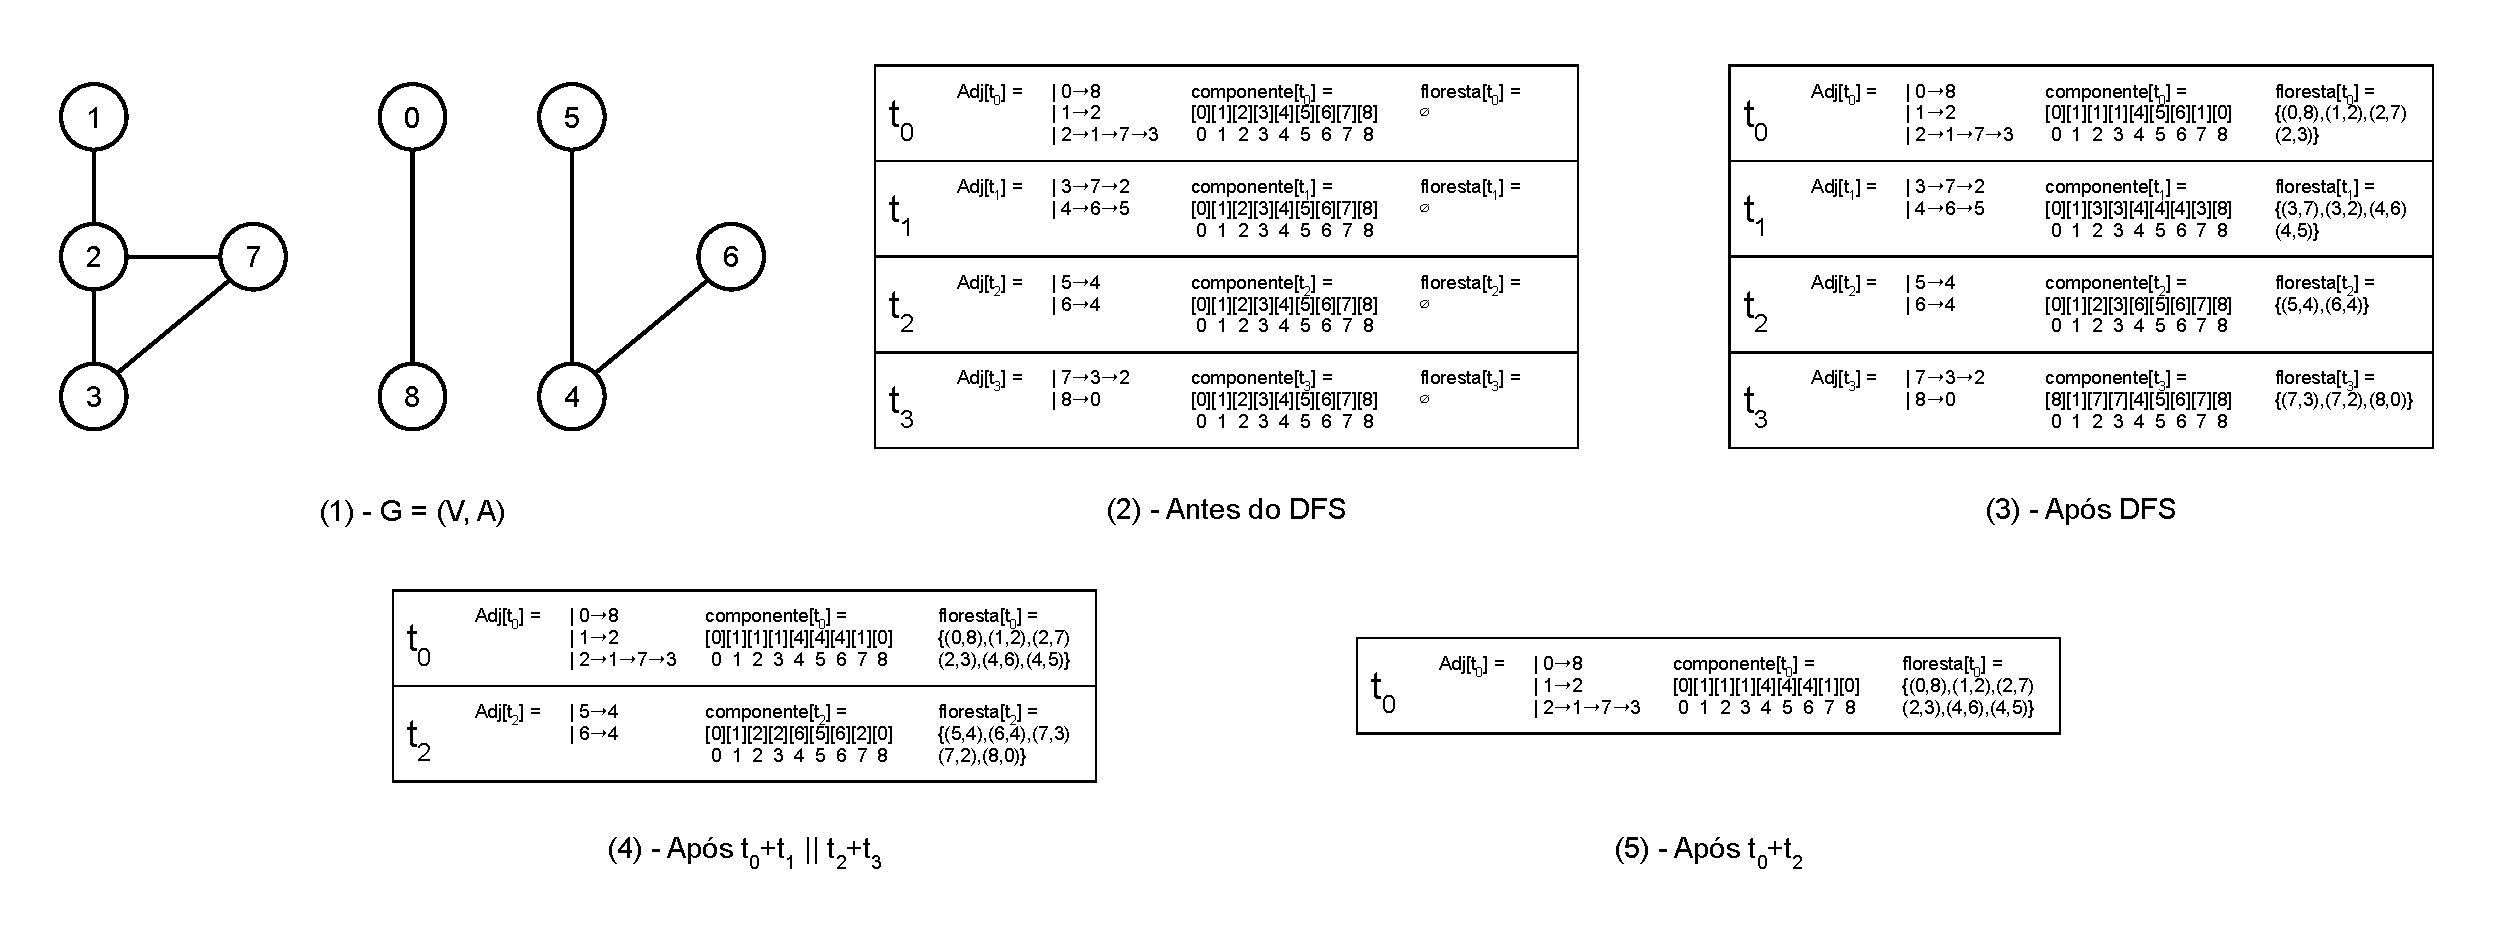
\includegraphics[width=1\textwidth]{tabela_exe_par.pdf}
\caption{Exemplo de Execução do Algoritmo 3}
\label{fig:alg3}
\end{figure}

{\color{gray}\lipsum[1]}

\begin{table}[h!]
    \resizebox{\textwidth}{!} { 
        \begin{tabular}{cccc}
		%THREAD0
			$t_0$ & 
		%LISTA
			$Adj[t_0]=\left\{\begin{tabular}{l}$0\to8$\\$1\to2$\\$2\to1\to7\to3$\end{tabular}\right.$ &
		%COMPONENTE
			\begin{tabular}{cccccccccc}
				\multicolumn{10}{l}{$componente[t_0]=$}\\
				%$_0$ & $_1$ & $_2$ & $_3$ & $_4$ & $_5$ & $_6$ & $_7$ & $_8$ & $_9$\\
				\hline
				\multicolumn{1}{|c|}{0} & \multicolumn{1}{c|}{1} & \multicolumn{1}{c|}{2} & 
				\multicolumn{1}{c|}{3} & \multicolumn{1}{c|}{4} & \multicolumn{1}{c|}{5} & 
				\multicolumn{1}{c|}{6} & \multicolumn{1}{c|}{7} & \multicolumn{1}{c|}{8} & 
				\multicolumn{1}{c|}{9}\\
				\hline
				\arrayrulecolor{white}\hline %pra dar um espacinho
				$^0$ & $^1$ & $^2$ & $^3$ & $^4$ & $^5$ & $^6$ & $^7$ & $^8$ & $^9$
			\end{tabular} & 
		%FLORESTA
			$\begin{tabular}{l}
				$floresta[t_0] =$\\
				\{(0,2), (0,3), (1,4)\}
			\end{tabular}$ \\
            %\hline
            %A&B&C&D\\ 
        \end{tabular}
  	}  
  	\caption{Exemplo de Execução do Algoritmo 3 [INACABADO]}
\end{table}

\section{Resultados e Análise}

\begin{figure}[h!]
	\begin{minipage}[b]{0.5\textwidth}
		\resizebox{\textwidth}{!}
		{
			        \begin{tabular}{cccc}
		%THREAD0
			$t_0$ & 
		%LISTA
			$Adj[t_0]=\left\{\begin{tabular}{l}$0\to8$\\$1\to2$\\$2\to1\to7\to3$\end{tabular}\right.$ &
		%COMPONENTE
			\begin{tabular}{cccccccccc}
				\multicolumn{10}{l}{$componente[t_0]=$}\\
				%$_0$ & $_1$ & $_2$ & $_3$ & $_4$ & $_5$ & $_6$ & $_7$ & $_8$ & $_9$\\
				\hline
				\multicolumn{1}{|c|}{0} & \multicolumn{1}{c|}{1} & \multicolumn{1}{c|}{2} & 
				\multicolumn{1}{c|}{3} & \multicolumn{1}{c|}{4} & \multicolumn{1}{c|}{5} & 
				\multicolumn{1}{c|}{6} & \multicolumn{1}{c|}{7} & \multicolumn{1}{c|}{8} & 
				\multicolumn{1}{c|}{9}\\
				\hline
				\arrayrulecolor{white}\hline %pra dar um espacinho
				$^0$ & $^1$ & $^2$ & $^3$ & $^4$ & $^5$ & $^6$ & $^7$ & $^8$ & $^9$
			\end{tabular} & 
		%FLORESTA
			$\begin{tabular}{l}
				$floresta[t_0] =$\\
				\{(0,2), (0,3), (1,4)\}
			\end{tabular}$ \\
            %\hline
            %A&B&C&D\\ 
        \end{tabular}
		}
	    \caption{entrada}
  	\end{minipage}
	\hfill
	\begin{minipage}[b]{0.5\textwidth}
		\resizebox{\textwidth}{!}
		{
			        \begin{tabular}{cccc}
		%THREAD0
			$t_0$ & 
		%LISTA
			$Adj[t_0]=\left\{\begin{tabular}{l}$0\to8$\\$1\to2$\\$2\to1\to7\to3$\end{tabular}\right.$ &
		%COMPONENTE
			\begin{tabular}{cccccccccc}
				\multicolumn{10}{l}{$componente[t_0]=$}\\
				%$_0$ & $_1$ & $_2$ & $_3$ & $_4$ & $_5$ & $_6$ & $_7$ & $_8$ & $_9$\\
				\hline
				\multicolumn{1}{|c|}{0} & \multicolumn{1}{c|}{1} & \multicolumn{1}{c|}{2} & 
				\multicolumn{1}{c|}{3} & \multicolumn{1}{c|}{4} & \multicolumn{1}{c|}{5} & 
				\multicolumn{1}{c|}{6} & \multicolumn{1}{c|}{7} & \multicolumn{1}{c|}{8} & 
				\multicolumn{1}{c|}{9}\\
				\hline
				\arrayrulecolor{white}\hline %pra dar um espacinho
				$^0$ & $^1$ & $^2$ & $^3$ & $^4$ & $^5$ & $^6$ & $^7$ & $^8$ & $^9$
			\end{tabular} & 
		%FLORESTA
			$\begin{tabular}{l}
				$floresta[t_0] =$\\
				\{(0,2), (0,3), (1,4)\}
			\end{tabular}$ \\
            %\hline
            %A&B&C&D\\ 
        \end{tabular}
		}
	    \caption{antes dfs}
  	\end{minipage}
\end{figure}

\begin{figure}[h!]
	\begin{minipage}[b]{0.5\textwidth}
		\resizebox{\textwidth}{!}
		{
			        \begin{tabular}{cccc}
		%THREAD0
			$t_0$ & 
		%LISTA
			$Adj[t_0]=\left\{\begin{tabular}{l}$0\to8$\\$1\to2$\\$2\to1\to7\to3$\end{tabular}\right.$ &
		%COMPONENTE
			\begin{tabular}{cccccccccc}
				\multicolumn{10}{l}{$componente[t_0]=$}\\
				%$_0$ & $_1$ & $_2$ & $_3$ & $_4$ & $_5$ & $_6$ & $_7$ & $_8$ & $_9$\\
				\hline
				\multicolumn{1}{|c|}{0} & \multicolumn{1}{c|}{1} & \multicolumn{1}{c|}{2} & 
				\multicolumn{1}{c|}{3} & \multicolumn{1}{c|}{4} & \multicolumn{1}{c|}{5} & 
				\multicolumn{1}{c|}{6} & \multicolumn{1}{c|}{7} & \multicolumn{1}{c|}{8} & 
				\multicolumn{1}{c|}{9}\\
				\hline
				\arrayrulecolor{white}\hline %pra dar um espacinho
				$^0$ & $^1$ & $^2$ & $^3$ & $^4$ & $^5$ & $^6$ & $^7$ & $^8$ & $^9$
			\end{tabular} & 
		%FLORESTA
			$\begin{tabular}{l}
				$floresta[t_0] =$\\
				\{(0,2), (0,3), (1,4)\}
			\end{tabular}$ \\
            %\hline
            %A&B&C&D\\ 
        \end{tabular}
		}
	    \caption{pós dfs}
  	\end{minipage}
  	\hfill
	\begin{minipage}[b]{0.5\textwidth}
		\resizebox{\textwidth}{!}
		{
			        \begin{tabular}{cccc}
		%THREAD0
			$t_0$ & 
		%LISTA
			$Adj[t_0]=\left\{\begin{tabular}{l}$0\to8$\\$1\to2$\\$2\to1\to7\to3$\end{tabular}\right.$ &
		%COMPONENTE
			\begin{tabular}{cccccccccc}
				\multicolumn{10}{l}{$componente[t_0]=$}\\
				%$_0$ & $_1$ & $_2$ & $_3$ & $_4$ & $_5$ & $_6$ & $_7$ & $_8$ & $_9$\\
				\hline
				\multicolumn{1}{|c|}{0} & \multicolumn{1}{c|}{1} & \multicolumn{1}{c|}{2} & 
				\multicolumn{1}{c|}{3} & \multicolumn{1}{c|}{4} & \multicolumn{1}{c|}{5} & 
				\multicolumn{1}{c|}{6} & \multicolumn{1}{c|}{7} & \multicolumn{1}{c|}{8} & 
				\multicolumn{1}{c|}{9}\\
				\hline
				\arrayrulecolor{white}\hline %pra dar um espacinho
				$^0$ & $^1$ & $^2$ & $^3$ & $^4$ & $^5$ & $^6$ & $^7$ & $^8$ & $^9$
			\end{tabular} & 
		%FLORESTA
			$\begin{tabular}{l}
				$floresta[t_0] =$\\
				\{(0,2), (0,3), (1,4)\}
			\end{tabular}$ \\
            %\hline
            %A&B&C&D\\ 
        \end{tabular}
		}
	    \caption{primeiro merge}
  	\end{minipage}
\end{figure}

\begin{figure}[h!]
	\centering
	\begin{minipage}[b]{0.5\textwidth}
		\resizebox{\textwidth}{!}
		{
			        \begin{tabular}{cccc}
		%THREAD0
			$t_0$ & 
		%LISTA
			$Adj[t_0]=\left\{\begin{tabular}{l}$0\to8$\\$1\to2$\\$2\to1\to7\to3$\end{tabular}\right.$ &
		%COMPONENTE
			\begin{tabular}{cccccccccc}
				\multicolumn{10}{l}{$componente[t_0]=$}\\
				%$_0$ & $_1$ & $_2$ & $_3$ & $_4$ & $_5$ & $_6$ & $_7$ & $_8$ & $_9$\\
				\hline
				\multicolumn{1}{|c|}{0} & \multicolumn{1}{c|}{1} & \multicolumn{1}{c|}{2} & 
				\multicolumn{1}{c|}{3} & \multicolumn{1}{c|}{4} & \multicolumn{1}{c|}{5} & 
				\multicolumn{1}{c|}{6} & \multicolumn{1}{c|}{7} & \multicolumn{1}{c|}{8} & 
				\multicolumn{1}{c|}{9}\\
				\hline
				\arrayrulecolor{white}\hline %pra dar um espacinho
				$^0$ & $^1$ & $^2$ & $^3$ & $^4$ & $^5$ & $^6$ & $^7$ & $^8$ & $^9$
			\end{tabular} & 
		%FLORESTA
			$\begin{tabular}{l}
				$floresta[t_0] =$\\
				\{(0,2), (0,3), (1,4)\}
			\end{tabular}$ \\
            %\hline
            %A&B&C&D\\ 
        \end{tabular}
		}
	    \caption{segundo merge}
  	\end{minipage}
\end{figure}

{\color{gray}\lipsum[1]}

\section{Conclusão}

{\color{gray}\lipsum[1]}

\bibliographystyle{sbc}
\bibliography{sbc-template}

\end{document}
